\documentclass[english]{article} 
\usepackage[absolute,overlay]{textpos} 
\usepackage{amsthm}
\usepackage{amsmath}
\usepackage{amssymb}
\usepackage[utf8]{inputenc}
\usepackage[english]{babel}
\usepackage{graphicx}
\usepackage{geometry}
\usepackage{caption}
\usepackage{subcaption}
\usepackage{pdfpages}
\usepackage{comment}
\usepackage{bm}
\usepackage{etoolbox}
\usepackage{mathtools}
\usepackage{tikz}

\usepackage{algpseudocode}
\usepackage{algorithm}
\usepackage{mathrsfs} 
\usepackage{multirow}

\usepackage{pgfplots}
\usepackage{pgfplotstable}
\usepackage{stmaryrd} 

\usepackage{hyperref}

\usepackage[noabbrev,capitalise]{cleveref}
\crefformat{appendix}{#2#1#3}

\usetikzlibrary{fillbetween}
\usepgfplotslibrary{fillbetween}

\usetikzlibrary{shapes.misc}
\usetikzlibrary{math} 

\usetikzlibrary{arrows}


\definecolor{darkspringgreen}{rgb}{0., 0.55, 0.3}
\definecolor{dartmouthgreen}{rgb}{0.05, 0.5, 0.06}
\definecolor{etonblue}{rgb}{0.59, 0.78, 0.64}
\definecolor{airforceblue}{rgb}{0., 0.4, 0.66}
\definecolor{arylideyellow}{rgb}{0.91, 0.84, 0.42}
\definecolor{emerald}{rgb}{0.31, 0.78, 0.47}
\definecolor{uclagold}{rgb}{1.0, 0.7, 0.0}
\definecolor{cadmiumorange}{rgb}{0.93, 0.53, 0.18}

\def\colorPalette{{"0.00 0.55 0.3","0.93 0.53 0.18","0.00 0.40 0.66","1.00 0.70 0.00","0.80 0.00 0.00","0.00 0.40 0.66", "0.05 0.50 0.06", "0.31 0.78 0.47", "0.59 0.78 0.64", "0.12 0.63 0.11", "0.75 0.43 0.1", "0.8 0.05 0.5"}}




%\newtheorem{theorem}{Theorem}
%\numberwithin{theorem}{section}
%\newtheorem{definition}{Definition}
%\numberwithin{definition}{section}
%\newtheorem{remark}{Remark}
%\numberwithin{remark}{section}
%\newtheorem{proposition}[theorem]{Proposition}
%\newtheorem{lemma}[theorem]{Lemma}
%\newtheorem{corollary}[theorem]{Corollary}

\theoremstyle{thmstyleone}
\newtheorem{theorem}{Theorem}
\newtheorem{proposition}[theorem]{Proposition}
\newtheorem{lemma}[theorem]{Lemma}
\newtheorem{corollary}[theorem]{Corollary}


\theoremstyle{thmstyletwo}
\newtheorem{example}{Example}
\newtheorem{remark}{Remark}

\theoremstyle{thmstylethree}
\newtheorem{definition}{Definition}


\newcommand{\lop}[0]{\mathcal{L}}
\newcommand{\lopd}[0]{\mathcal{L}_\Delta}
\newcommand{\lopdt}[0]{\mathcal{L}_{\Delta}}
\newcommand{\LL}{\lopdt}
\newcommand{\usol}[0]{\underline{\uvec{u}}_\Delta}
\newcommand{\usoldt}[0]{\underline{\uvec{u}}_\Delta}


\newcommand{\up}[0]{\underline{\uvec{u}}^{(p)}}

\newcommand{\usoldto}[0]{\tilde{\underline{\uvec{u}}}_\Delta}

\newcommand{\uapp}[0]{\uvec{u}_h}
\newcommand{\wapp}[0]{w_h}

\newcommand{\massmatrix}[0]{\mathcal{M}}

\newcommand{\tess}[0]{\mathcal{T}_h}


\newcommand{\uvec}[2][3]{\boldsymbol{#2\mkern-#1mu}\mkern#1mu}


\newcommand{\res}[0]{\textbf{R}}
\newcommand\norm[1]{\left\lVert#1\right\rVert}
\newcommand\abs[1]{\left\lvert#1\right\rvert}

\newcommand{\flux}[0]{\boldsymbol{F}}
\newcommand{\source}[0]{\boldsymbol{S}}
\newcommand{\ST}[0]{\boldsymbol{ST}_i^K}
\newcommand{\extra}[0]{\boldsymbol{ST}_i}


\newcommand{\elres}[0]{\uvec{\Phi}^K(\uapp)}
\newcommand{\noderes}[0]{\uvec{\Phi}^K_i(\uapp)}
%\newcommand{\spacestuff}[0]{\boldsymbol{\phi}_i}
\newcommand{\cund}[0]{\underline{\uvec{c}}}
\newcommand{\lopdi}[0]{\mathcal{L}_{\Delta,i}}
\newcommand{\csoldt}[0]{\underline{\uvec{c}}_\Delta}
\newcommand{\basis}[0]{\uvec{v}}
\newcommand{\mis}[0]{\mu}
\def\restriction#1#2{\mathchoice
              {\setbox1\hbox{${\displaystyle #1}_{\scriptstyle #2}$}
              \restrictionaux{#1}{#2}}
              {\setbox1\hbox{${\textstyle #1}_{\scriptstyle #2}$}
              \restrictionaux{#1}{#2}}
              {\setbox1\hbox{${\scriptstyle #1}_{\scriptscriptstyle #2}$}
              \restrictionaux{#1}{#2}}
              {\setbox1\hbox{${\scriptscriptstyle #1}_{\scriptscriptstyle #2}$}
              \restrictionaux{#1}{#2}}}
\def\restrictionaux#1#2{{#1\,\smash{\vrule height .8\ht1 depth .85\dp1}}_{\,#2}} 
\newcommand\swapifbranches[3]{#1{#3}{#2}}
\newcommand{\R}{\mathbb{R}}
\newcommand{\dt}{\Delta t}
\newcommand{\redun}[1]{{\color{red} {\large \textit{Is the following redundant?}} #1}}
\newcommand{\davide}[1]{{\color{purple}#1}}
\newcommand{\lore}[1]{ \textbf{{\color{blue}#1}}}
\newcommand{\question}[1]{{\color{red} \large Question: #1 }}
\newcommand{\bu}{\uvec{u}}
\newcommand{\bbu}{\underline{\uvec{u}}}
\newcommand{\bU}{\uvec{U}}
\newcommand{\bbU}{\underline{\uvec{U}}}
\newcommand{\bbr}{\underline{\uvec{r}}}
\newcommand{\by}{\uvec{y}}
\newcommand{\bby}{\underline{\uvec{y}}}
\newcommand{\bG}{{\uvec{G}}}
\newcommand{\bbt}{\underline{t}}
\newcommand{\vecz}{\underline{0}}
\newcommand{\matz}{\underline{\underline{0}}}
\newcommand{\vecbeta}{\underline{\beta}}
\newcommand{\CIP}{\text{CIP}}
\newcommand{\OSS}{\text{OSS}}
\newcommand{\CFL}{\text{CFL}}

\newcommand{\undu}{\underline{\uvec{u}}}
\newcommand{\undy}{\underline{\uvec{y}}}
\newcommand{\undspacetilde}{\widetilde{\underline{\uvec{\phi}}}}
\newcommand{\spacestuff}{\uvec{\phi}}
\newcommand{\undv}{\underline{\uvec{v}}}
\newcommand{\undw}{\underline{\uvec{w}}}
\newcommand{\undr}{\underline{\uvec{r}}}
\newcommand{\undz}{\underline{\uvec{z}}}
\newcommand{\lopdtp}[0]{\mathcal{L}_{\Delta,p}}
\newcommand{\usolp}[0]{\underline{\uvec{u}}_{\Delta}^{(p)}}
\newcommand{\Xp}[0]{X^{(p)}}
\newcommand{\Yp}[0]{Y^{(p)}}
\newcommand{\uex}[0]{\underline{\uvec{u}}_{ex}}
\newcommand{\uexp}[0]{\underline{\uvec{u}}_{ex}^{(p)}}
\newcommand{\lopdLp}[0]{\mathcal{L}_\Delta^{1,(p)}}
\newcommand{\lopdHp}[0]{\mathcal{L}_\Delta^{2,(p)}}
\newcommand{\embep}[0]{\mathcal{E}^{(p)}}
\newcommand{\projp}[0]{\Pi^{(p)}}
\newcommand{\trialspace}[1]{\varphi_{#1}} %phi space _i
\newcommand{\trialspaceiter}[2]{\varphi_{#1}^{#2}} %phi space _i
\newcommand{\trialtime}[1]{\psi^{#1}} %psi time ^m
\newcommand{\trialtimeiter}[2]{\psi^{#1,#2}} %psi time ^m
%THE FOLLOWING IS  ^l TO AVOID CONFUSION WITH u_n
\newcommand{\trialspacetime}[1]{\vartheta^{#1}} %theta space time 
\newcommand{\trialspacetimeiter}[2]{\vartheta^{#1,#2}}

%ADER-FV
\newcommand{\trialspaceFVp}[1]{\varphi_{#1}} %predictor
\newcommand{\trialspaceFVc}[1]{\lambda_{#1}} %corrector 
\newcommand{\APNPM}{{ADER-$\mathbb P_N \mathbb P_M$ }}

%Temperature
%\newcommand{\Temp}{\tau}
\newcommand{\Temp}{T}


\newcommand{\E}{\boldsymbol{E}}

\newcommand{\pnpm}[2]{\mathbb P_{#1}\mathbb P_{#2}}  %PNPM schemes

\newcommand{\RIcolor}[1]{{\leavevmode\color{black} #1}}
\newcommand{\RIIcolor}[1]{{\leavevmode\color{black} #1}}


%\DeclarePairedDelimiter\abs{\lvert}{\rvert}

\newcommand{\hpsi}{\widehat{\psi}}
\newcommand{\hphi}{\widehat{\varphi}}
\newcommand{\hl}{\widehat{\lambda}}
\newcommand{\hK}{\widehat{K}}
\newcommand{\hw}{\widehat{\omega}}

\newcommand{\xt}{\uvec{x},t}
\newcommand{\et}{\uvec{xi},t}

\begin{document}
\author{L. Micalizzi\footnote{Affiliation: Institute of Mathematics, University of Zurich, Winterthurerstrasse 190, Zurich, 8057, Switzerland. Email: lorenzo.micalizzi@math.uzh.ch.} }
\title{Spectral methods for Lagrangian Continuous FEM}  


\maketitle
%\tableofcontents

\abstract{bla bla}

\section{Convention on the transformation}
Let us consider a space domain occupying a region $\Omega_0\subseteq \mathbb{R}^2$ at time $t=0$. Its general point is denoted by $\uvec{X}\in \Omega_0$.
%
Then, we assume the existence of a map $\uvec{x}=\widetilde{\uvec{x}}(\uvec{X},t)$, associating to each $\uvec{X}$ a point $\uvec{x}\in \Omega_t$, where $\Omega_t\subseteq \mathbb{R}^2$ is the image of $\Omega_0$ through $\widetilde{\uvec{x}}(\cdot,t)$.

Actually, for convenience, we will not work with the map $\widetilde{\uvec{x}}(\cdot,t):\Omega_0\rightarrow\Omega_t$, from the initial configuration $\Omega_0$ to $\Omega_t$, but rather with $\uvec{x}(\cdot,t):\widehat{\Omega}\rightarrow\Omega_t$, from a reference configuration $\widehat{\Omega}$ to $\Omega_t$.
The general point in $\widehat{\Omega}$ is denoted by $\uvec{\xi}$.
%
A sketch is reported in Figure \ref{fig:lagrangian_maps}.
%
\begin{figure}
	\centering
	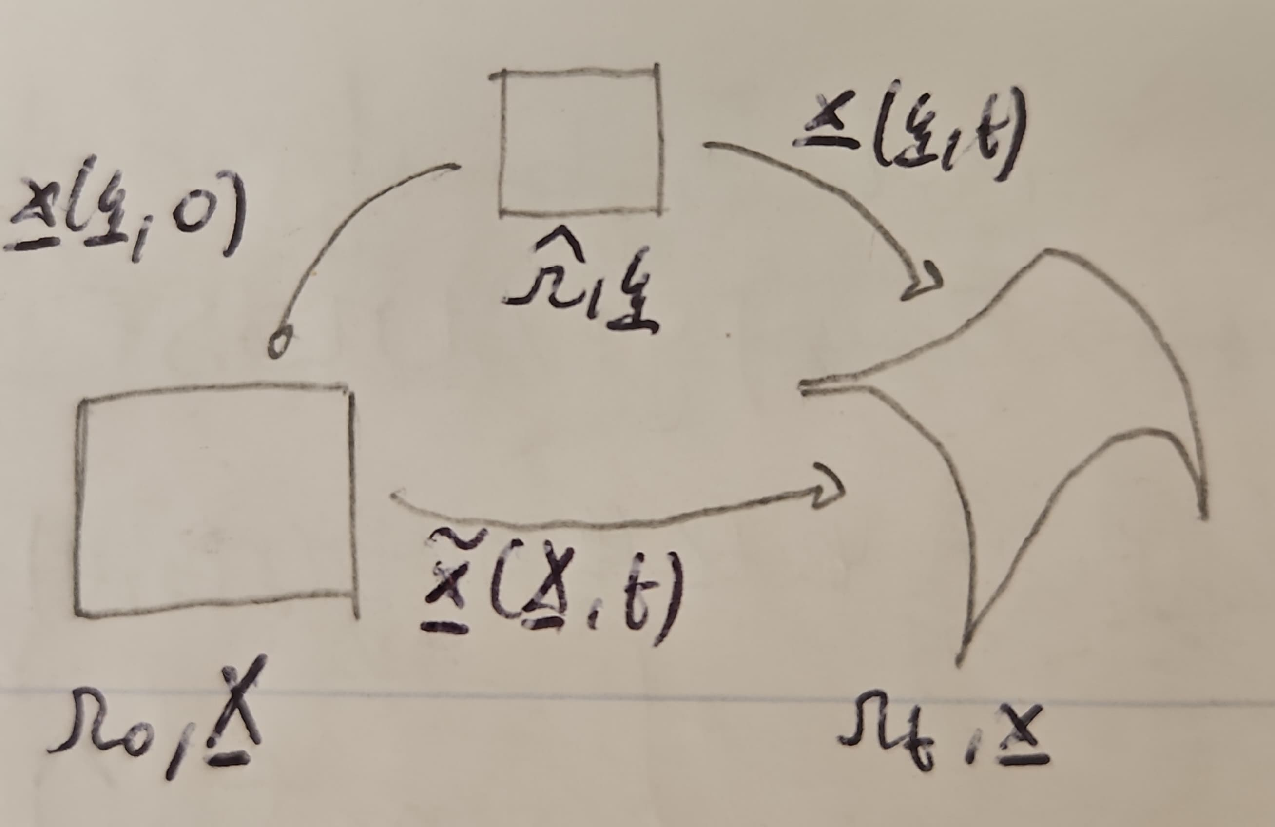
\includegraphics[width=0.4\textwidth]{lagrangian_maps.pdf}
	\caption{Sketch of the maps $\widetilde{\uvec{x}}(\uvec{X},t)$ and $\uvec{x}(\uvec{\xi},t)$}\label{fig:lagrangian_maps}
\end{figure}
%
Further, we define the deformation gradient $\uvec{J}(\uvec{\xi},t):=\nabla_{\uvec{\xi}}\uvec{x}(\uvec{\xi},t).$



\textcolor{red}{Summarizing, I work with a map $\uvec{x}(\uvec{\xi},t)$ from the reference configuration $\widehat{\Omega}$ to $\Omega_t$.}


\section{Governing equations}
The governing equations are
\begin{itemize}
\item \textbf{Deformation map}
\begin{equation}
\frac{d}{dt}\uvec{x}(\uvec{\xi},t)=\uvec{v}(\uvec{x}(\uvec{\xi},t),t);
\end{equation}

\item \textbf{Mass conservation}

\begin{align}
&H(\uvec{x}(\uvec{\xi},t),t)=\frac{\widehat{H}(\uvec{\xi})}{det \uvec{J}(\uvec{\xi},0)} ,\text{ or} \label{eq:strong_mass_conservation}\\
&\frac{d}{dt}H(\uvec{x},t)+H(\uvec{x},t)div_{\uvec{x}}\uvec{v}(\uvec{x},t)=0; \label{eq:weak_mass_conservation}
\end{align}

\item \textbf{Momentum conservation}
\begin{align}
&H\frac{d}{dt}\uvec{v}(\uvec{x},t)+\nabla_{\uvec{x}}\left(\frac{gH^2(\uvec{x},t)}{2}\right)+gH(\uvec{x},t)\nabla_{\uvec{x}}B(\uvec{x})=\uvec{0} ,\text{ or}, \label{eq:momentum_non_wb}\\
&\frac{d}{dt}\uvec{v}(\uvec{x},t)+g\nabla_{\uvec{x}}\left(H(\uvec{x},t)+B(\uvec{x})\right)=\uvec{0}. \label{eq:momentum_wb}
\end{align}


\textcolor{red}{NB: for me $H$ is the water height, $B$ is the bathymetry.}



\end{itemize}


\section{Discretization}
The discretization of Dobrev, Tzanio and Rieben is assumed.
The thermodynamic variable $H_h$ is approximated in a discontinuous space of piecewise polynomial functions $\hpsi_i$ of degree $M$. Locally, we have
\begin{equation}
H_h(\uvec{\xi},t):=\sum_{i}H_i(t)\hpsi(\uvec{\xi}),
\end{equation}

The kinetic variables $\uvec{x}_h$ and $\uvec{v}_h$ are approximated in a continuous space of piecewise polynomial functions $\hphi_i$ of degree $M+1$. Globally, we have
\begin{align}
\uvec{x}_h(\uvec{\xi},t)&:=\sum_{i}\uvec{x}_i(t)\hphi(\uvec{\xi}),\\
\uvec{v}_h(\uvec{\xi},t)&:=\sum_{i}\uvec{v}_i(t)\hphi(\uvec{\xi}),
\end{align}


We define the basis functions on the trajectory of the motions $\psi(\uvec{x},t)$ and $\varphi(\uvec{x},t)$, in such a way that they are constant along the characteristics of the particles
\begin{align}
\varphi(\uvec{x},t)&:=\hphi(\uvec{\xi}(\uvec{x},t)),\\
\psi(\uvec{x},t)&:=\hpsi(\uvec{\xi}(\uvec{x},t)).
\end{align}

This allows to define the spatial description of the discretized variables
\begin{align}
H_h(\uvec{x},t)&:=\sum_{i}H_i(t)\psi(\uvec{x},t)=\sum_{i}H_i(t)\hpsi(\uvec{\xi}(\uvec{x},t)),\\
\uvec{x}_h(\uvec{x},t)&:=\sum_{i}\uvec{x}_i(t)\varphi(\uvec{x},t)=\sum_{i}\uvec{x}_i(t)\hphi(\uvec{\xi}(\uvec{x},t)),\\
\uvec{v}_h(\uvec{x},t)&:=\sum_{i}\uvec{v}_i(t)\varphi(\uvec{x},t)=\sum_{i}\uvec{v}_i(t)\hphi(\uvec{\xi}(\uvec{x},t)),
\end{align}
denoted, with abuse of notation, with the same symbols.



\section{Main point}\label{sec:main_point}
\textcolor{red}{
Q: Is it possible to achieve a proper mass lumping in Lagrangian, by adopting some spectral approach (special nodal bases with associated nodes used as quadrature points), e.g. Lagrange polynomials in the Gauss--Lobatto (GL) points?\\
A: Yes, BUT the (lumped) matrices will depend on time.
}

We set $\lambda$ as a general handler for $\psi$ and $\varphi$ and we have
\begin{align}
\begin{split}
\int_{K(t)} \lambda_i(\uvec{x},t)\lambda_j(\uvec{x},t)d\uvec{x}&=\int_{K(t)} \hl_i(\uvec{\xi},t)\hl_j(\uvec{\xi},t) det \uvec{J}(\uvec{\xi},t) d\uvec{\xi}\\
&=\int_{\widehat{K}} \hl_i(\uvec{\xi},t)\hl_j(\uvec{\xi},t) det \uvec{J}(\uvec{\xi},t) d\uvec{\xi}\\
&\approx \delta_{i,j}\widehat{\omega}_i det \uvec{J}(\uvec{\xi}_i,t)=M_{\lambda_i}^K(t).
\end{split}
\end{align}

\textcolor{red}{
NB: This is not the matrix that one integrates in Lagrangian, because one has usually to do with $\int_K H\lambda_i\lambda_j$.
However, in SW, $H$ can be removed, see for example \eqref{eq:weak_mass_conservation} or \eqref{eq:momentum_wb}. Indeed, we can put it back by multiplying the equations by $H$.
NEVERTHELESS, the lumping makes also the matrix $\int_K H\lambda_i\lambda_j$, which should be constant if one integrated it exactly, time-dependent.}

\begin{align}
\begin{split}
\int_{K(t)}H(\uvec{x},t) \lambda_i(\uvec{x},t)\lambda_j(\uvec{x},t)d\uvec{x}&=\int_{K(t)} \hl_i(\uvec{\xi},t)\hl_j(\uvec{\xi},t) det \uvec{J}(\uvec{\xi},t) d\uvec{\xi}\\
&=\int_{\widehat{K}}H(\uvec{\xi},t) \hl_i(\uvec{\xi},t)\hl_j(\uvec{\xi},t) det \uvec{J}(\uvec{\xi},t) d\uvec{\xi}\\
&\approx \delta_{i,j}H_i(t)\widehat{\omega}_i det \uvec{J}(\uvec{\xi}_i,t)=H_i(t)M_{\lambda_i}^K(t).
\end{split}
\end{align}

A time-dependent matrix may be a problem BUT, in the end, with the lumping it is just a point evaluation and becomes part of the ODE at the RHS!


\textcolor{blue}{QUESTION $1$: Do you think that this is dangerous?}


\section{Discrete equations}


\begin{itemize}
\item \textbf{Deformation map}
NO DOUBT

\begin{equation}
\frac{d}{dt}\uvec{x}_i(t)=\uvec{v}_i(t);
\end{equation}

Moreover, it is WB.


\item \textbf{Mass conservation}

\begin{align}
&H(\uvec{x}(\uvec{\xi},t),t)=\frac{\widehat{H}(\uvec{\xi})}{det \uvec{J}(\uvec{\xi},0)} ,\text{ or} \label{eq:strong_mass_conservation_bis}\\
&\frac{d}{dt}H(\uvec{x},t)+H(\uvec{x},t)div_{\uvec{x}}\uvec{v}(\uvec{x},t)=0; \label{eq:weak_mass_conservation_bis}
\end{align}

\textcolor{blue}{
QUESTION $2$: I kind of think that \eqref{eq:strong_mass_conservation_bis} is naturally WB even if it does not look so but tell me if I'm wrong. In fact, if $\uvec{v}_i=0$ at the beginning, $\uvec{x}(\uvec{\xi},0)$ is the classical Eulerian linear mapping and $H_h(\uvec{x},t)+B_h(\uvec{x},t)\equiv const$ for lake at rest. Am I right?\\
%
Even though I do not think it is necessary, I could consider a weak formulation of the second one with discontinuous test function $\psi_i$, apply the divergence theorem to guarantee coupling between the cells and I would end up with some $(H\uvec{v})^*$ on the boundary, coming from some Riemann solver. It is in principle not $0$ but it's not a big deal. There are WB Riemann solvers making sure to have $(H\uvec{v})^*=0$ in lake at rest. We used one with Mario in the staggered project\footnote{BTW Mario, we have to come back on that, I've been very busy as well!}.
}

\item \textbf{Momentum conservation}
\begin{align}
&H\frac{d}{dt}\uvec{v}(\uvec{x},t)+\nabla_{\uvec{x}}\left(\frac{gH^2(\uvec{x},t)}{2}\right)+gH(\uvec{x},t)\nabla_{\uvec{x}}B(\uvec{x})=\uvec{0} ,\text{ or}, \label{eq:momentum_non_wb_bis}\\
&\frac{d}{dt}\uvec{v}(\uvec{x},t)+g\nabla_{\uvec{x}}\left(H(\uvec{x},t)+B(\uvec{x})\right)=\uvec{0}. \label{eq:momentum_wb_bis}
\end{align}
\end{itemize}


Here, I need a proper weak formulation: I can consider both \eqref{eq:momentum_non_wb_bis} or \eqref{eq:momentum_wb_bis}, in any case as I showed in Section \ref{sec:main_point}, I will have a time dependent lumped mass matrix BUT this is not a problem because it is just a point evaluation. So, I consider \eqref{eq:momentum_wb_bis}, which is easier to be made WB, and I get

\begin{equation}
\sum_{K \in K_i} M^K_{\varphi_i}(t)\frac{d}{dt}\uvec{v}_i(t)-g \sum_{K \in K_i} \int_K (H_h+B_h)\nabla_{\uvec{x}} \varphi_i d\uvec{x}=\uvec{0},
\end{equation}
leading to
\begin{equation}
\frac{d}{dt}\uvec{v}_i(t)=\frac{1}{M_{\varphi_i}(t)}g \sum_{K \in K_i} \int_K (H_h+B_h)\nabla_{\uvec{x}} \varphi_i d\uvec{x},
\end{equation}
with $M_{\varphi_i}(t)=\sum_{K \in K_i} M^K_{\varphi_i}(t)$, which is WB.


\textcolor{red}{
NB: For me $K_i$ is the set of the elements containing the DoF $\uvec{x}_i$, which is well defined because we do not allow for connectivity changes.
}



\textcolor{blue}{
QUESTION $3$: The boundary integral vanished because of the continuity of $\varphi_i$ and its compact support. So I have no coupling between cells. Mario, in staggered we had something like
%!*-----------------------------------------------------
%!*I need to add now Mario's extra terms
%ConservationElement(2:3)=ConservationElement(2:3) &
%                        & + 0.5_DP* grav * ( ustar(1)**2-u_inside(1)**2 ) * n(:) * ev%weight_edge(k,iq) &  !*1/2*g[(h*)^2-h^2]*nu
%                        & + grav * 0.5_DP * ( ustar(1)+u_inside(1) ) * (b_star - b_inside) * n(:) * ev%weight_edge(k,iq) !*g(h+h*)/2*(b*-b)
%!*-----------------------------------------------------
\begin{align}
\begin{split}
\uvec{CT}_K(\uvec{u}_h):=\frac{1}{2}g\int_{\partial K}  \left( (H^*)^2-H_h\vert_K^2 \right) \uvec{\nu} d \uvec{\sigma}+\frac{1}{2}g\int_{\partial K}  \left( (H^*)+H_h\vert_K \right)\left( (B^*)-B_h\vert_K \right) \uvec{\nu} d \uvec{\sigma}.
\end{split}
\label{eq:CT}
\end{align}
Would it work here? I should probably multiply by $\varphi_i$...
}



\section{Stabilization}
\textcolor{blue}{
QUESTION $4$: Burman?
\begin{align}
\uvec{ST}_i(\uapp)=\sum_f\sum_{r=1}^R \alpha_{f,r} \Bigg\llbracket \frac{\partial^r}{\partial x^r} \varphi_i \Bigg\rrbracket \cdot \Bigg\llbracket \frac{\partial^r}{\partial x^r} \begin{pmatrix}
\eta_h\\
v_h
\end{pmatrix} \Bigg\rrbracket  , \quad \eta_h=H_h+B_h
\label{eq:jt}
\end{align}
Maybe, we can even adapt
\begin{align}
\textbf{ST}_i(\uapp)=\sum_{f}\alpha_f  \Bigg\llbracket \uvec{J}  \frac{\partial}{\partial x} \varphi_i \Bigg\rrbracket \mathcal{B}_f \Bigg\llbracket \uvec{J}\frac{\partial}{\partial x} \uvec{u}_h-\boldsymbol{S}^* \Bigg\rrbracket, \quad \boldsymbol{S}^*=-\begin{pmatrix}
0\\
gH_h \frac{\partial}{\partial x}B_h
\end{pmatrix} 
\label{eq:jr}
\end{align}
where $\uvec{J}=\frac{\partial \uvec{F}}{\partial \uvec{u}}$.
%
The first is easier. For shocks we do a blending with Lax-Friedrichs. I'd like to avoid $\beta$ stabilization, because it did not work for arbitrary high order in Eulerian.
%
}

\section{If it works}

\begin{itemize}

\item[•] It is truly arbitrary high order because we do not have the problem with Bernstein and $\beta$

\item[•] It is extendible to Euler

\item[•] It is extendible to multi-D, in the code here they have quads so one can work with PGL and tensor products.

\item[•] One can use whatever time integration method.

\end{itemize}

\bibliography{sn-bibliography}
\bibliographystyle{plain}



\end{document}
